\documentclass[tikz,border=1.25mm]{standalone}
\usetikzlibrary{matrix, positioning, shapes, fit, shapes.geometric, backgrounds, arrows.meta}
\usepackage{amssymb}

\definecolor{kellygreen}{rgb}{0.3, 0.73, 0.09}
\definecolor{gray}{rgb}{0.54, 0.54, 0.54}
\definecolor{slate}{rgb}{0.094,0.094,0.094}
\definecolor{cobalt}{rgb}{0.244,0.364,0.972}

\begin{document}

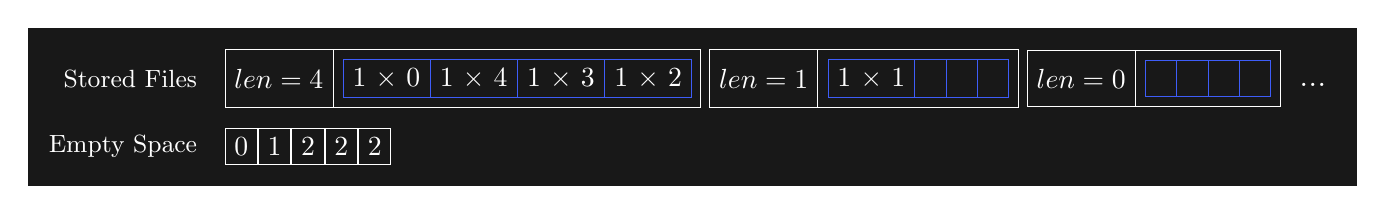
\begin{tikzpicture}[
  background rectangle/.style={fill=slate},
  show background rectangle,
  every node/.style={
    color=white,
    draw,
    minimum height=4.6mm,
  }
]

\matrix(m1)[
  matrix anchor=north west,
  matrix of nodes,
  nodes in empty cells,
  column sep=1mm,
  draw=none,
] {
  \node[rectangle split, rectangle split horizontal, rectangle split parts=2, draw]{
    \nodepart{one} $len=4$
    \nodepart{two} \tikz{\node[rectangle split, rectangle split horizontal, rectangle split parts=4, draw, color=cobalt, text=white]{
        \nodepart{one} 1 $\times$ 0
        \nodepart{two} 1 $\times$ 4
        \nodepart{three} 1 $\times$ 3
        \nodepart{four} 1 $\times$ 2
    }}
  }; &
  \node[rectangle split, rectangle split horizontal, rectangle split parts=2, draw]{
    \nodepart{one} $len=1$
    \nodepart{two} \tikz{\node[rectangle split, rectangle split horizontal, rectangle split parts=4, draw, color=cobalt, text=white]{
        \nodepart{one} 1 $\times$ 1
    }}
  }; &
  \node[rectangle split, rectangle split horizontal, rectangle split parts=2, draw]{
    \nodepart{one} $len=0$
    \nodepart{two} \tikz{\node[rectangle split, rectangle split horizontal, rectangle split parts=4, draw, color=cobalt, text=white]{}}
  }; & |[shift={(0mm,0.25mm)},draw=none,text depth=-1mm,inner ysep=2mm]| \hspace{-1mm} \large{...} \\
};

\matrix(m2)[
  below=10mm of m1.north west,
  matrix anchor=north west,
  matrix of nodes,
  nodes in empty cells,
  draw=none
] {
  0 & 1 & 2 & 2 & 2 \\
};

\node[draw=none, left=1mm of m1]{\small{Stored Files}};
\node[draw=none, left=1mm of m2]{\small{Empty Space}};

\end{tikzpicture}

\end{document}
